\documentclass[a4paper,12pt,twoside]{memoir}

% Castellano
\usepackage[spanish,es-tabla]{babel}
\selectlanguage{spanish}
\usepackage[utf8]{inputenc}
\usepackage[T1]{fontenc}
\usepackage{lmodern} % scalable font
\usepackage{microtype}
\usepackage{placeins}

\RequirePackage{booktabs}
\RequirePackage[table]{xcolor}
\RequirePackage{xtab}
\RequirePackage{multirow}

% Links
\usepackage[colorlinks]{hyperref}
\hypersetup{
	allcolors = {red}
}

% Ecuaciones
\usepackage{amsmath}

% Rutas de fichero / paquete
\newcommand{\ruta}[1]{{\sffamily #1}}

% Párrafos
\nonzeroparskip


% Imagenes
\usepackage{graphicx}
\newcommand{\imagen}[2]{
	\begin{figure}[!h]
		\centering
		\includegraphics[width=0.9\textwidth]{#1}
		\caption{#2}\label{fig:#1}
	\end{figure}
	\FloatBarrier
}

\newcommand{\imagenflotante}[2]{
	\begin{figure}%[!h]
		\centering
		\includegraphics[width=0.9\textwidth]{#1}
		\caption{#2}\label{fig:#1}
	\end{figure}
}



% El comando \figura nos permite insertar figuras comodamente, y utilizando
% siempre el mismo formato. Los parametros son:
% 1 -> Porcentaje del ancho de página que ocupará la figura (de 0 a 1)
% 2 --> Fichero de la imagen
% 3 --> Texto a pie de imagen
% 4 --> Etiqueta (label) para referencias
% 5 --> Opciones que queramos pasarle al \includegraphics
% 6 --> Opciones de posicionamiento a pasarle a \begin{figure}
\newcommand{\figuraConPosicion}[6]{%
  \setlength{\anchoFloat}{#1\textwidth}%
  \addtolength{\anchoFloat}{-4\fboxsep}%
  \setlength{\anchoFigura}{\anchoFloat}%
  \begin{figure}[#6]
    \begin{center}%
      \Ovalbox{%
        \begin{minipage}{\anchoFloat}%
          \begin{center}%
            \includegraphics[width=\anchoFigura,#5]{#2}%
            \caption{#3}%
            \label{#4}%
          \end{center}%
        \end{minipage}
      }%
    \end{center}%
  \end{figure}%
}

%
% Comando para incluir imágenes en formato apaisado (sin marco).
\newcommand{\figuraApaisadaSinMarco}[5]{%
  \begin{figure}%
    \begin{center}%
    \includegraphics[angle=90,height=#1\textheight,#5]{#2}%
    \caption{#3}%
    \label{#4}%
    \end{center}%
  \end{figure}%
}
% Para las tablas
\newcommand{\otoprule}{\midrule [\heavyrulewidth]}
%
% Nuevo comando para tablas pequeñas (menos de una página).
\newcommand{\tablaSmall}[5]{%
 \begin{table}
  \begin{center}
   \rowcolors {2}{gray!35}{}
   \begin{tabular}{#2}
    \toprule
    #4
    \otoprule
    #5
    \bottomrule
   \end{tabular}
   \caption{#1}
   \label{tabla:#3}
  \end{center}
 \end{table}
}

%
%Para el float H de tablaSmallSinColores
\usepackage{float}

%
% Nuevo comando para tablas pequeñas (menos de una página).
\newcommand{\tablaSmallSinColores}[5]{%
 \begin{table}[H]
  \begin{center}
   \begin{tabular}{#2}
    \toprule
    #4
    \otoprule
    #5
    \bottomrule
   \end{tabular}
   \caption{#1}
   \label{tabla:#3}
  \end{center}
 \end{table}
}

\newcommand{\tablaApaisadaSmall}[5]{%
\begin{landscape}
  \begin{table}
   \begin{center}
    \rowcolors {2}{gray!35}{}
    \begin{tabular}{#2}
     \toprule
     #4
     \otoprule
     #5
     \bottomrule
    \end{tabular}
    \caption{#1}
    \label{tabla:#3}
   \end{center}
  \end{table}
\end{landscape}
}

%
% Nuevo comando para tablas grandes con cabecera y filas alternas coloreadas en gris.
\newcommand{\tabla}[6]{%
  \begin{center}
    \tablefirsthead{
      \toprule
      #5
      \otoprule
    }
    \tablehead{
      \multicolumn{#3}{l}{\small\sl continúa desde la página anterior}\\
      \toprule
      #5
      \otoprule
    }
    \tabletail{
      \hline
      \multicolumn{#3}{r}{\small\sl continúa en la página siguiente}\\
    }
    \tablelasttail{
      \hline
    }
    \bottomcaption{#1}
    \rowcolors {2}{gray!35}{}
    \begin{xtabular}{#2}
      #6
      \bottomrule
    \end{xtabular}
    \label{tabla:#4}
  \end{center}
}

%
% Nuevo comando para tablas grandes con cabecera.
\newcommand{\tablaSinColores}[6]{%
  \begin{center}
    \tablefirsthead{
      \toprule
      #5
      \otoprule
    }
    \tablehead{
      \multicolumn{#3}{l}{\small\sl continúa desde la página anterior}\\
      \toprule
      #5
      \otoprule
    }
    \tabletail{
      \hline
      \multicolumn{#3}{r}{\small\sl continúa en la página siguiente}\\
    }
    \tablelasttail{
      \hline
    }
    \bottomcaption{#1}
    \begin{xtabular}{#2}
      #6
      \bottomrule
    \end{xtabular}
    \label{tabla:#4}
  \end{center}
}

%
% Nuevo comando para tablas grandes sin cabecera.
\newcommand{\tablaSinCabecera}[5]{%
  \begin{center}
    \tablefirsthead{
      \toprule
    }
    \tablehead{
      \multicolumn{#3}{l}{\small\sl continúa desde la página anterior}\\
      \hline
    }
    \tabletail{
      \hline
      \multicolumn{#3}{r}{\small\sl continúa en la página siguiente}\\
    }
    \tablelasttail{
      \hline
    }
    \bottomcaption{#1}
  \begin{xtabular}{#2}
    #5
   \bottomrule
  \end{xtabular}
  \label{tabla:#4}
  \end{center}
}



\definecolor{cgoLight}{HTML}{EEEEEE}
\definecolor{cgoExtralight}{HTML}{FFFFFF}

%
% Nuevo comando para tablas grandes sin cabecera.
\newcommand{\tablaSinCabeceraConBandas}[5]{%
  \begin{center}
    \tablefirsthead{
      \toprule
    }
    \tablehead{
      \multicolumn{#3}{l}{\small\sl continúa desde la página anterior}\\
      \hline
    }
    \tabletail{
      \hline
      \multicolumn{#3}{r}{\small\sl continúa en la página siguiente}\\
    }
    \tablelasttail{
      \hline
    }
    \bottomcaption{#1}
    \rowcolors[]{1}{cgoExtralight}{cgoLight}

  \begin{xtabular}{#2}
    #5
   \bottomrule
  \end{xtabular}
  \label{tabla:#4}
  \end{center}
}




\graphicspath{ {./img/} }

% Capítulos
\chapterstyle{bianchi}
\newcommand{\capitulo}[2]{
	\setcounter{chapter}{#1}
	\setcounter{section}{0}
	\chapter*{#2}
	\addcontentsline{toc}{chapter}{#2}
	\markboth{#2}{#2}
}

% Apéndices
\renewcommand{\appendixname}{Apéndice}
\renewcommand*\cftappendixname{\appendixname}

\newcommand{\apendice}[1]{
	%\renewcommand{\thechapter}{A}
	\chapter{#1}
}

\renewcommand*\cftappendixname{\appendixname\ }

% Formato de portada
\makeatletter
\usepackage{xcolor}
\newcommand{\tutor}[1]{\def\@tutor{#1}}
\newcommand{\course}[1]{\def\@course{#1}}
\definecolor{cpardoBox}{HTML}{E6E6FF}
\def\maketitle{
  \null
  \thispagestyle{empty}
  % Cabecera ----------------
\noindent
\includegraphics[width=\textwidth]{cabecera}\vspace{1cm}%
  \vfill
  % Título proyecto y escudo informática ----------------
  \colorbox{cpardoBox}{%
    \begin{minipage}{.8\textwidth}
      \vspace{.5cm}\Large
      \begin{center}
      \textbf{TFG del Grado en Ingeniería Informática}\vspace{.6cm}\\
      \textbf{\LARGE\@title{}}
      \end{center}
      \vspace{.2cm}
    \end{minipage}

  }%
  \hfill\begin{minipage}{.20\textwidth}
    
\includegraphics[width=\textwidth]{escudoInfor}
  \end{minipage}
  \vfill
  % Datos de alumno, curso y tutores ------------------
  \begin{center}%
  {%
    \noindent\LARGE
    Presentado por \@author{}\\ 
    en Universidad de Burgos --- \@date{}\\
    Tutor: \@tutor{}\\
  }%
  \end{center}%
  \null
  \cleardoublepage
  }
\makeatother


% Datos de portada
\title{título del TFG \\Documentación Técnica}
\author{nombre alumno}
\tutor{nombre tutor}
\date{\today}

\begin{document}

\maketitle



\cleardoublepage



%%%%%%%%%%%%%%%%%%%%%%%%%%%%%%%%%%%%%%%%%%%%%%%%%%%%%%%%%%%%%%%%%%%%%%%%%%%%%%%%%%%%%%%%



\frontmatter


\clearpage

% Indices
\tableofcontents

\clearpage

\listoffigures

\clearpage

\listoftables

\clearpage

\mainmatter

\appendix

\apendice{Plan de Proyecto Software}

\section{Introducción}

\section{Planificación temporal}

\section{Estudio de viabilidad}

\subsection{Viabilidad económica}

\subsection{Viabilidad legal}



\apendice{Especificación de Requisitos}

\section{Introducción}

\section{Objetivos generales}

\section{Catalogo de requisitos}

\section{Especificación de requisitos}



\apendice{Especificación de diseño}

\section{Introducción}

En esta sección se describe cómo están implementados los datos de esta aplicación, cuáles son los procedimientos más relevantes y cómo se organizan los proyectos.

\section{Diseño de datos}

En esta sección, explicaremos como están organizados tanto el conjunto de imágenes obtenidas, cómo son y como se organizan las características extraídas de las imágenes, y el diagrama de clases de la aplicación.

\subsection{Conjunto de imágenes}

El conjunto de imágenes es el descrito en \cite{GDXray:imagenes}. Estas imágenes están disponibles en un repositorio público: \url{https://drive.google.com/drive/folders/143893UAlc7TB_ZiTGlg9S9w4rp3wHlji}. Este repositorio contiene 5 grupos de carpetas una para cada grupo: \textit{Castings}, \textit{Welds}, \textit{Baggage}, \textit{Nature} y \textit{Settings}. Estas imágenes son almacenadas en formato de escala de grises de 8 bits ``png'' (\textit{Portable Network Graphics}). También tenemos metadatos adicionales para cada serie en un archivo ASCII llamado Xssss\_readme.txt incluido en la subcarpeta Xssss, donde ``X'' es la inicial del grupo y ``ssss'' es el número de serie del grupo de imágenes. Para este proyecto sólo hemos utilizado el grupo \textit{Castings}.

En \cite{GDXray:imagenes} este grupo se describe como: ``(...)contiene 2.727 imágenes de rayos-x organizadas en 67 series. Las imágenes de rayos-x se tomaron principalmente de partes automotrices (ruedas de aluminio y nudillos) usando un intensificador de imágenes. (...)Es interesante resaltar que la serie C0001 contiene no solo una secuencia de 72 imágenes de rayos-x tomadas de una rueda de aluminio girando su eje central, pero también anotaciones de \textit{Bounding Boxes} de la verdad del terreno (\textit{ground truth}) de 226 pequeños defectos y la matriz de calibración de cada imagen que relaciona las coordenadas 3D de la rueda de aluminio con coordenadas 2D de la imagen de rayos-x'' (p.4-p.5).

\subsection{Diagrama de clases de la aplicación}

En este apartado se comentará las clases realizadas por nosotros en el proyecto. Es decir, las clases que se han creado para realizar la aplicación. Señalamos que, únicamente se analizaran las realizadas por nosotros, toda la estructura del repositorio \texttt{metal-defect-detection} \cite{metal-defect-detection:repositorio} no será analizada.

\subsubsection{Clases de la aplicación}

Para la aplicación se han creado las siguientes clases:

\begin{itemize}
    \item \texttt{XrayDataset} dentro de \texttt{app.py}: Clase que contiene el conjunto de datos de las imágenes de rayos-X, tiene una sola función que crea un conjunto de datos compuesto por una imagen con su id, su directorio, su altura y su anchura también crean una clase ``\textit{Casting Defect}'' que es el tipo de defectos que puede haber.
    \item \texttt{Detector} dentro de \texttt{app.py}: Clase que contiene toda la estructura gráfica de la ventada de la aplicación. Se inicializan todos los elementos gráficos (\textit{frames}, botones...), las variables necesarias para cada uno, y los mediadores. También contiene todos los métodos necesarios para la visualización de las imágenes, la detección de los defectos y la visualización de las máscaras y la información adicional de los defectos. Debido a que todo se encuentra en la misma clase la mayoría de funciones no devuelve nada.
    \item \texttt{InferenceConfig} dentro de \texttt{app.py}: Clase que contiene únicamente dos variables para la configuración del \texttt{config}. Esta configuración hace que se ejecute la detección de defectos en una solo imagen cada vez.
\end{itemize}

\imagen{diagrama_clases}{Diagrama de clases}

\section{Diseño procedimental}

\subsection{Diagramas de secuencia}

En este apartado se mostrarán los diagramas de secuencia respectivos a 4 tareas de la aplicación:

\begin{itemize}
    \item Cargar de imágenes, ver figura \ref{DS_carga}.
    \item Predecir los defectos de las imágenes y mostrar la imagen con los defectos, ver figura \ref{DS_predecir}.
    \item Visualizar la información de los defectos, ver figura \ref{DS_info}.
    \item Visualizar las máscaras de los defectos, ver figura \ref{DS_masks}.
\end{itemize}

\newpage

\begin{figure}[H]
	\centering
	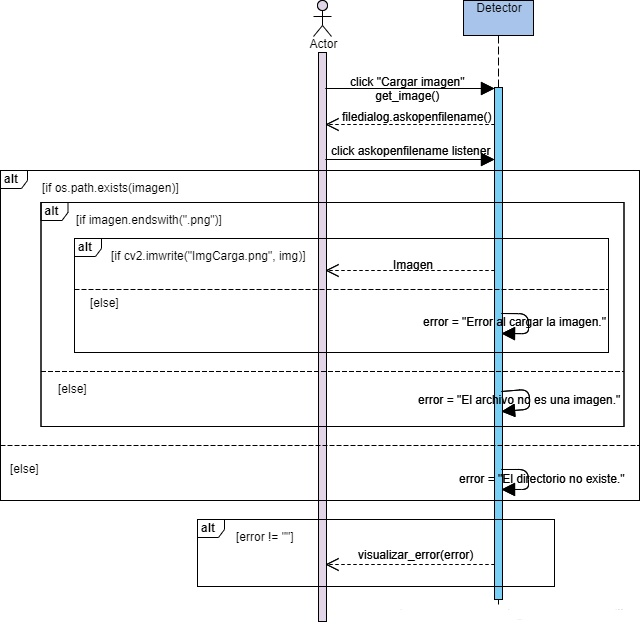
\includegraphics[scale=0.7]{DS_carga}
	\caption{Diagrama de secuencia para la cargar una imagen}
	\label{DS_carga}
\end{figure}

\begin{figure}[H]
	\centering
	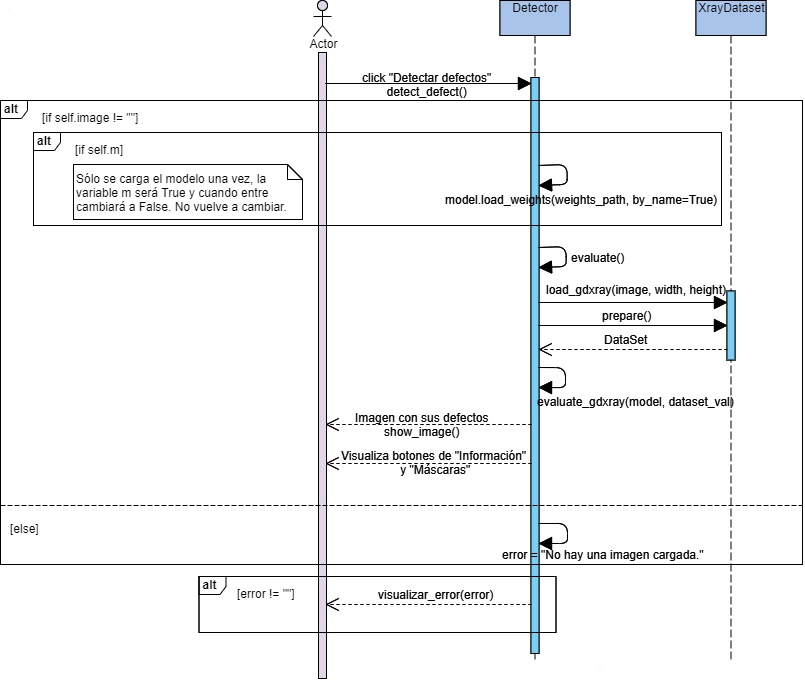
\includegraphics[scale=0.6]{DS_predecir}
	\caption{Diagrama de secuencia para la predicción y muestra de defectos}
	\label{DS_predecir}
\end{figure}

\begin{figure}[H]
	\centering
	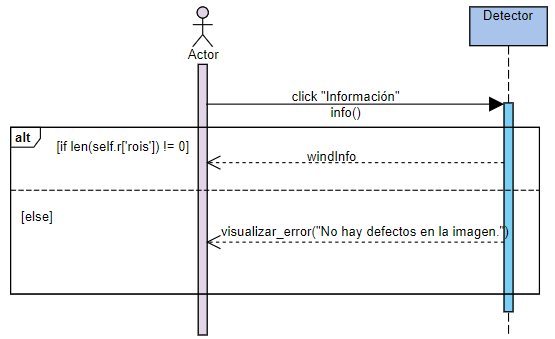
\includegraphics[scale=0.9]{DS_info}
	\caption{Diagrama de secuencia para la muestra de la información de los defectos}
	\label{DS_info}
\end{figure}

\begin{figure}[H]
	\centering
	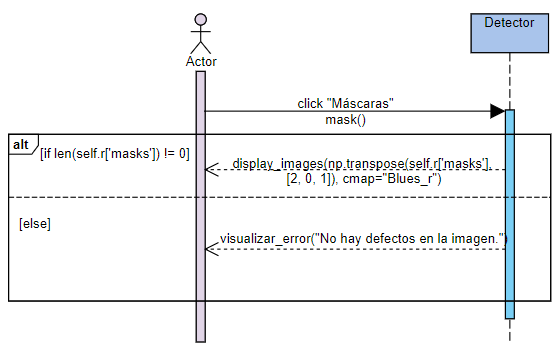
\includegraphics[scale=0.9]{DS_masks}
	\caption{Diagrama de secuencia para la muestra de las máscaras de los defectos}
	\label{DS_masks}
\end{figure}

\section{Diseño arquitectónico}

En este apartado se definirá el diseño arquitectónico de la aplicación, la cual sigue el patrón de diseño \textit{Singleton}.

\subsection{Patrón Singleton}

El patrón de diseño \textit{Singleton} \cite{singleton} (instancia única) está diseñado para restringir la creación de objetos pertenecientes a una clase o el valor de un tipo a un único objeto. Su intención consiste en garantizar que una clase sólo tenga una instancia y proporcionar un punto de acceso global a ella. No se encarga de la creación de objetos en sí, sino que se enfoca en la restricción en la creación de un objeto.
\apendice{Documentación técnica de programación}

\section{Introducción}

\section{Estructura de directorios}

\section{Manual del programador}

\section{Compilación, instalación y ejecución del proyecto}

\section{Pruebas del sistema}

\apendice{Documentación de usuario}

\section{Introducción}

En esta sección explicaremos lo necesario para que los usuarios puedan instalar y utilizar la aplicación.

\section{Requisitos de usuarios}

El usuario, para poder utilizar la aplicación, deberá tener instalado \textit{Python}, al menos la versión 3.6.8 y cargar el entorno virtual que se ha creado con la ayuda del archivo \texttt{environment.yml}. Idealmente, el sistema se instalará en Windows 10, ya que la aplicación está optimizada para este sistema operativo.

\section{Instalación}

Los pasos para la instalación del proyecto se detallan en \nameref{instalacion}. Les resumimos:

\begin{itemize}
    \item Primero compruebe que ha descargado todos los archivos como indica el apartado \label{descargar}.
    \item Cree el entorno virtual y actívelo.
    \item Compruebe que las bibliotecas de OpenCV y TensorFlow se han instalado correctamente, si no es así instálelas en el entorno.
\end{itemize}

Para ejecutar la aplicación:
\begin{itemize}
    \item python app.py
\end{itemize}

\section{Manual del usuario}

En esta sección se describe como realizar las diferentes operaciones de la aplicación.

\subsection{Cargar imagen}

Para cargar una imagen:

\begin{enumerate}
    \item Hacer click en el botón ``Cargar imagen''.
    \item Seleccionar una imagen del dispositivo.
    \item La imagen aparecerá en la aplicación.
\end{enumerate}

\begin{figure}[H]
	\centering
	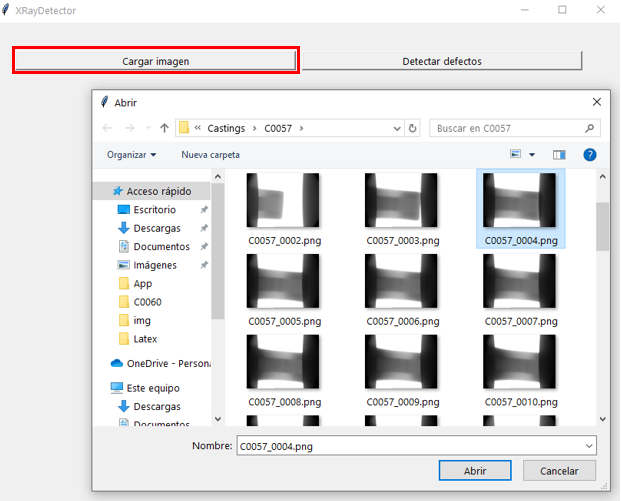
\includegraphics[scale=0.8]{carga_imagen}
	\caption{Carga de una imagen en la aplicación}
	\label{carga_imagen}
\end{figure}

\subsection{Detectar defectos}

Para detectar los defectos de la imagen cargada:

\begin{enumerate}
    \item Hacer click en el botón ``Detectar defectos''.
    \item Espere, el proceso puede tardar unos segundos.
    \item La imagen con los defectos aparecerá en la aplicación.
\end{enumerate}

\imagen{detectar_defectos}{Detectar defectos de una imagen\label{detectar_defectos}}

\newpage

\subsection{Visualizar máscaras}

Para visualizar las máscaras de la imagen:

\begin{enumerate}
    \item Hacer click en el botón ``Máscaras''.
    \item Se abre una segunda ventana con la/s imágenes de las máscaras.
\end{enumerate}

\begin{figure}[H]
	\centering
	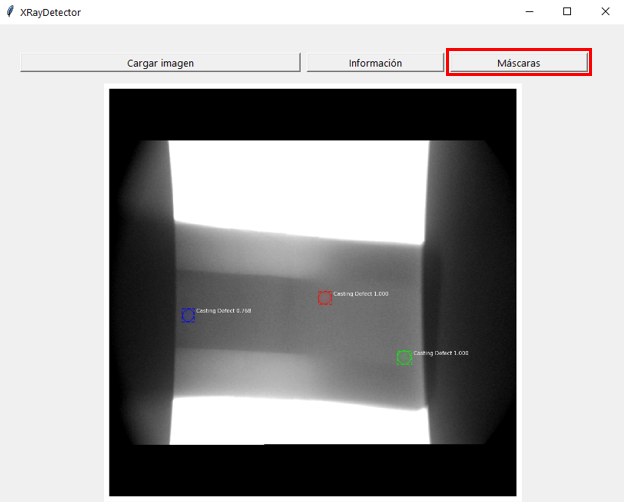
\includegraphics[scale=0.7]{visualizar_mascaras}
	\caption{Visualizar las máscaras de los defectos de la imagen}
	\label{visualizar_mascaras}
\end{figure}

\imagen{mascara_cargada}{Máscaras de los defectos de la imagen\label{mascara_cargada}}

\subsection{Información de los defectos}

Para ver la información sobre los defectos detectados en la imagen:

\begin{enumerate}
    \item Hacer click en el botón ``Información''.
    \item Se abre una segunda ventana con la información de los defectos.
\end{enumerate}

\imagen{informacion_defectos}{Visualizar la información de los defectos de la imagen\label{informacion_defectos}}

\begin{figure}[htb]
	\centering
	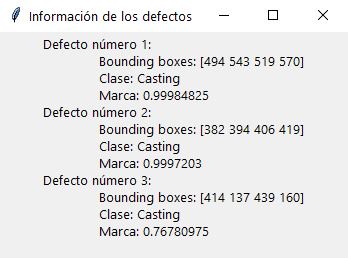
\includegraphics[width=0.53\textwidth]{informacion_cargada}
	\caption{Información de los defectos de la imagen}
	\label{informacion_cargada}
\end{figure}

\newpage

\subsection{Errores}

Los errores controlados que pueden salir son:

\begin{enumerate}
    \item Se produce algún problema al cargar la imagen, mensaje: ``Error al cargar la imagen.''. Ver figura \ref{error_carga}.
    \item Se carga un archivo que no es una imagen, mensaje: ``El archivo no es una imagen.''. Ver figura \ref{archivo_no_imagen}.
    \item Se selecciona un directorio que no existe, mensaje: ``El directorio no existe.''. Ver figura \ref{no_existe_directorio}.
    \item Se hace click en el botón ``Detectar defectos'' sin haber cagado la imagen, mensaje: ``No hay una imagen cargada.''. Ver figura \ref{no_imagen_cargada}.
    \item Se produce algún problema al cargar la imagen después de detectar los defectos, mensaje: ``Error al cargar la imagen.''. Ver figura \ref{error_carga}.
    \item No haya defectos en la imagen y se hace click en el botón ``Máscaras'', mensaje: ``No hay defectos en la imagen.''. Ver figura \ref{no_defectos}.
    \item No haya defectos en la imagen y se hace click en el botón ``Información'', mensaje: ``No hay defectos en la imagen.''. Ver figura \ref{no_defectos}.
\end{enumerate}

\begin{figure}[htb]
	\centering
	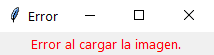
\includegraphics[width=0.7\textwidth]{error_carga}
	\caption{Problema al cargar la imagen}
	\label{error_carga}
\end{figure}

\begin{figure}[htb]
	\centering
	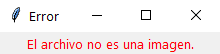
\includegraphics[width=0.7\textwidth]{archivo_no_imagen}
	\caption{El archivo cargado no es una imagen}
	\label{archivo_no_imagen}
\end{figure}

\begin{figure}[htb]
	\centering
	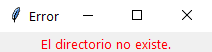
\includegraphics[width=0.7\textwidth]{no_existe_directorio}
	\caption{No existe el directorio seleccionado}
	\label{no_existe_directorio}
\end{figure}

\begin{figure}[htb]
	\centering
	
\includegraphics[width=0.7\textwidth]{no_imagen_cargada}
	\caption{No hay una imagen cargada para detectar defectos}
	\label{no_imagen_cargada}
\end{figure}

\begin{figure}[htb]
	\centering
	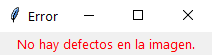
\includegraphics[width=0.7\textwidth]{no_defectos}
	\caption{No hay defectos detectados en la imagen}
	\label{no_defectos}
\end{figure}


\bibliographystyle{plain}
\bibliography{bibliografiaAnexos}

\end{document}
